\documentclass[11pt,a4paper]{article}
\usepackage[T1]{fontenc}\usepackage{lmodern}\usepackage[margin=2.2cm]{geometry}\usepackage{microtype}
\usepackage{booktabs}\usepackage{tabularx}\usepackage{longtable}\usepackage{array}\usepackage{float}
\usepackage{caption}\usepackage{enumitem}\usepackage{xcolor}\usepackage{amsmath}
\usepackage{pgfplots}\pgfplotsset{compat=1.18}\usepgfplotslibrary{groupplots}
\usepackage[colorlinks=true,linkcolor=blue!50!black,urlcolor=blue!50!black]{hyperref}
\definecolor{seriesA}{HTML}{2A78D6}\definecolor{seriesB}{HTML}{EB6834}\definecolor{seriesC}{HTML}{3BA272}
\captionsetup{font=small,labelfont=bf}\setlist{itemsep=2pt,topsep=4pt}\setlength{\emergencystretch}{3em}
\newcolumntype{Y}{>{\raggedright\arraybackslash}X}
\pgfplotsset{every axis/.append style={axis line style={draw=black!40}, tick style={draw=black!40},
  ymajorgrids, grid style={draw=black!12}, legend style={draw=none, font=\small}}}
\title{\textbf{Hybrid Video Provenance Framework (HVPF)}\\[3pt]\large Phase 3 Results: Vision Transformer, Ensembles and PRNU Injection into AI Video}
\author{Talha Aslam\\ MS Thesis}
\date{12 October 2026}
\begin{document}\maketitle
\begin{abstract}\noindent
Phase 3 adds a Vision Transformer on I-frame noise residuals, calibrated models, model ensembles and
equal-length inputs for the sequence models. It also adds a harder attack, taken from Khan et al.\ (2025):
a real camera's PRNU injected into AI-generated video, so that the clip passes conventional PRNU verification.
As in Phase 2, the task is a three-class decision for each video clip (organic / manipulated / synthetic),
compared with the conventional PRNU method (PCE rule).
All numbers are generated directly from the result files.
\end{abstract}
\section{Key results}\begin{itemize}
\item \textbf{Best result:} Stacking (LR) reaches macro F1 0.851, PVA 0.836 and authentic-vs-not AUC 0.941 (EER 0.149) in 5-fold cross-validation on camera models never seen in training (Phase 2 best: XGBoost, F1 0.792). The conventional PCE rule reaches AUC 0.549 (RQ3); it dropped from Phase 2 because injected AI clips pass it.
\item \textbf{Vision Transformer:} the best single model (F1 0.820) and by far the most robust on unseen sources: it recognises 90\% of FloreView genuine videos (XGBoost 55\%), including stabilised phones without a usable PRNU (Table~\ref{tab:cross}). Plain averaging of all models (F1 0.814) does not beat the ViT alone; stacking, which learns how much to trust each model, does (0.851).
\item \textbf{Calibration is not worth it:} per-class threshold offsets change macro F1 on the test cameras by +0.004 (XGBoost) but cost PVA on unseen sources (XGBoost -5, ViT -4 points). Stacking, also fitted on validation data, is the best combination on both (Table~\ref{tab:cal}).
\item \textbf{PRNU injected into AI video (Khan-style):} 2,984 AI clips carry a real camera's PRNU. At full strength the PCE rule accepts 98\% of them as genuine footage of that camera (96\% for unseen generators); stacking accepts 0\% (1\%) (Table~\ref{tab:khanai}).
\item \textbf{Weakest spots:} (1) AI clips from unseen generators that were also WhatsApp-like compressed: stacking calls 42\% synthetic, 42\% manipulated and 16\% organic. (2) Genuine VISION videos that went through our own re-encoding: stacking recognises 45\% of them (15\% of the WhatsApp-like ones); almost all others are called manipulated, because the attacked clips went through the same encoder (Table~\ref{tab:cond}).
\item \textbf{10 frames:} with equal-length inputs, 10 frames is slightly better than 5 even on length-matched clips (+1 to +2 PVA points); combinations of the Step 8 models at 10 frames reach F1 0.844 without the ViT, so a 10-frame ViT and stack is the next likely gain.
\item \textbf{Features (RQ1):} removing Noiseprint statistics costs the most (about 0.05 macro F1), followed by TSNCS and PRNU (0.01--0.03); FFT and residual moments add almost nothing (Figure~\ref{fig:ablation}).
\end{itemize}
\section{What changed in Phase 3}\begin{itemize}
\item \textbf{Vision Transformer (Step 8b).} Pretrained ViT-S/16 (21.7M parameters, ImageNet-21k) fine-tuned on three SRM high-pass residuals of each I-frame (random 224$\times$224 crops and flips, AdamW, mixed precision, class-balanced loss, early stopping on validation macro F1). A clip's prediction averages its first five I-frames $\times$ four crops. This is the same input size as PDC-ViT.
\item \textbf{Calibration and ensembles (Step 8c).} Validation predictions of every model are now kept. \emph{+cal}: three class offsets on the log-probabilities tuned for validation macro F1. \emph{Ensembles}: mean class probability of SVM+XGB, of the three sequence models, of all learned models, and of the three best models on validation data; \emph{stacking}: logistic regression on all models' validation outputs. Validation data always comes from other camera models than the test data.
\item \textbf{Equal-length inputs.} Clips shorter than the window repeat their own frames, so sequence models cannot use the number of I-frames as a shortcut (a Phase 2 limitation).
\item \textbf{Wider tuning.} XGBoost: depth 4/6/8 and a min-child-weight variant, up to 1500 trees; SVM: $C$ up to 30.
\item \textbf{Harder synthetic class.} Khan-style AI clips with an injected camera PRNU ($\alpha$ = 0.5 and 1, same strength units as the manipulation attacks) are added to training and test. The attacker estimates the fingerprint from the camera's own natural videos, never from the analyst's reference videos. Cameras without a usable video PRNU are not impersonated.
\end{itemize}
\section{Data and protocol}
The evaluation uses 27,583 clips. Model inputs come from the first five I-frames of each clip. Results are averaged over five grouped cross-validation folds: no camera model is in both training and test. \emph{Realistic} uses all clips; \emph{encoder-controlled} uses only clips encoded by our libx264 pipeline (genuine re-encodes, attacks, AI clips), so encoder traces cannot separate the classes. \emph{Cross-dataset} is FloreView (genuine) plus GenBuster (unseen AI generators), tested with the fixed-split models.
\begin{table}[H]\centering\small\caption{Clips per class and source.}\begin{tabular}{llr}\toprule Class & Source & Clips \\\midrule
AI + injected camera PRNU & GenBuster & 1,200 \\
AI + injected camera PRNU & GenVidBench & 1,784 \\
manipulated & VISION-attack & 7,200 \\
organic & ACID & 4,380 \\
organic & ACID-attack & 3,168 \\
organic & FloreView & 1,716 \\
organic & VISION & 1,259 \\
organic & VISION-attack & 2,400 \\
synthetic & GenBuster & 1,800 \\
synthetic & GenVidBench & 2,676 \\
\bottomrule\end{tabular}\end{table}
\section{Main results}
\begin{table}[H]\centering\small\setlength{\tabcolsep}{4pt}\caption{Realistic setup, 5-fold cross-validation (mean $\pm$ std over folds), 5 frames. PVA = share of clips assigned to their true provenance class; AUC/EER for genuine vs not genuine. Lower block: calibrated models and combinations (Step 8c).}\label{tab:main}\begin{tabular}{lccccc}\toprule Model & PVA & Macro F1 & AUC (3-class) & AUC genuine vs not & EER \\\midrule
PCE rule & -- & -- & -- & 0.549 & 0.449 \\
SVM & 0.765 $\pm$ 0.025 & 0.769 $\pm$ 0.025 & 0.898 & 0.884 & 0.201 \\
XGBoost & 0.791 $\pm$ 0.030 & 0.794 $\pm$ 0.029 & 0.927 & 0.913 & 0.177 \\
GRU & 0.773 $\pm$ 0.027 & 0.779 $\pm$ 0.022 & 0.919 & 0.906 & 0.190 \\
1D-CNN & 0.768 $\pm$ 0.029 & 0.774 $\pm$ 0.022 & 0.910 & 0.895 & 0.197 \\
Transformer & 0.770 $\pm$ 0.027 & 0.780 $\pm$ 0.024 & 0.916 & 0.902 & 0.194 \\
ViT (residual) & 0.806 $\pm$ 0.020 & 0.820 $\pm$ 0.017 & 0.933 & 0.912 & 0.182 \\
\midrule
Ens.\ SVM+XGB & 0.789 $\pm$ 0.025 & 0.794 $\pm$ 0.022 & 0.926 & 0.912 & 0.179 \\
Ens.\ GRU+CNN+Transf. & 0.784 $\pm$ 0.027 & 0.793 $\pm$ 0.022 & 0.924 & 0.912 & 0.182 \\
Ens.\ all & 0.807 $\pm$ 0.026 & 0.814 $\pm$ 0.022 & 0.941 & 0.927 & 0.167 \\
Ens.\ top-3 (val) & 0.818 $\pm$ 0.025 & 0.827 $\pm$ 0.019 & 0.946 & 0.932 & 0.161 \\
Stacking (LR) & 0.836 $\pm$ 0.019 & 0.851 $\pm$ 0.014 & 0.955 & 0.941 & 0.149 \\
XGBoost + cal. & 0.787 $\pm$ 0.032 & 0.797 $\pm$ 0.028 & 0.927 & 0.913 & 0.178 \\
Ens.\ all + cal. & 0.804 $\pm$ 0.027 & 0.814 $\pm$ 0.020 & 0.940 & 0.927 & 0.168 \\
Ens.\ top-3 (val) + cal. & 0.812 $\pm$ 0.026 & 0.826 $\pm$ 0.019 & 0.946 & 0.932 & 0.162 \\
\bottomrule\end{tabular}\end{table}
\begin{table}[H]\centering\small\caption{Encoder-controlled setup (5-fold) and cross-dataset test (FloreView + GenBuster), 5 frames.}\begin{tabular}{lcccccc}\toprule & \multicolumn{3}{c}{Encoder-controlled} & \multicolumn{3}{c}{Cross-dataset} \\\cmidrule(lr){2-4}\cmidrule(lr){5-7} Model & PVA (\%) & Macro F1 & AUC & PVA (\%) & Macro F1 & AUC \\\midrule
PCE rule & -- & -- & 0.513 & -- & -- & 0.406 \\
SVM & 74 & 0.751 & 0.860 & 56 & 0.630 & 0.793 \\
XGBoost & 76 & 0.768 & 0.886 & 64 & 0.728 & 0.922 \\
GRU & 75 & 0.756 & 0.876 & 53 & 0.619 & 0.825 \\
1D-CNN & 75 & 0.758 & 0.872 & 60 & 0.660 & 0.844 \\
Transformer & 75 & 0.756 & 0.872 & 60 & 0.715 & 0.889 \\
ViT (residual) & 75 & 0.763 & 0.856 & 82 & 0.842 & 0.942 \\
\midrule Ens.\ SVM+XGB & 76 & 0.770 & 0.886 & 60 & 0.667 & 0.884 \\
Ens.\ GRU+CNN+Transf. & 76 & 0.769 & 0.884 & 59 & 0.683 & 0.866 \\
Ens.\ all & 78 & 0.785 & 0.898 & 64 & 0.722 & 0.913 \\
Ens.\ top-3 (val) & 78 & 0.789 & 0.897 & 70 & 0.776 & 0.944 \\
Stacking (LR) & 81 & 0.816 & 0.906 & 82 & 0.863 & 0.965 \\
XGBoost + cal. & 76 & 0.774 & 0.887 & 59 & 0.698 & 0.919 \\
Ens.\ all + cal. & 78 & 0.792 & 0.899 & 60 & 0.703 & 0.904 \\
Ens.\ top-3 (val) + cal. & 78 & 0.792 & 0.897 & 67 & 0.759 & 0.943 \\
\bottomrule\end{tabular}\end{table}
\begin{table}[H]\centering\small\caption{Phase 2 vs Phase 3 (realistic, 5-fold, 5 frames). Phase 3 also contains the injected AI clips, so its test set is larger and harder.}\begin{tabular}{lcccccc}\toprule & \multicolumn{2}{c}{PVA (\%)} & \multicolumn{2}{c}{Macro F1} & \multicolumn{2}{c}{AUC genuine vs not} \\\cmidrule(lr){2-3}\cmidrule(lr){4-5}\cmidrule(lr){6-7} Model & Phase 2 & Phase 3 & Phase 2 & Phase 3 & Phase 2 & Phase 3 \\\midrule
PCE rule & -- & -- & -- & -- & 0.635 & 0.549 \\
XGBoost & 78 & 79 & 0.792 & 0.794 & 0.899 & 0.913 \\
GRU & 77 & 77 & 0.785 & 0.779 & 0.891 & 0.906 \\
Transformer & 76 & 77 & 0.775 & 0.780 & 0.880 & 0.902 \\
\midrule Best model & 78 & 84 & 0.792 & 0.851 & 0.899 & 0.941 \\
\bottomrule\end{tabular}\end{table}
\section{Calibration and ensembles on unseen sources}
Calibration moves the decision thresholds to where they work best on the validation cameras. That barely helps on test cameras from the same datasets, and FloreView phones and unseen AI generators look different, so the moved thresholds hurt there. Stacking is also fitted on validation data, but it learns how much weight each model gets (the ViT, the most robust model on unseen sources, is one of them) and is the best combination on both. Fixed split, 5 frames:
\begin{table}[H]\centering\small\caption{Effect of calibration and combination: same datasets vs unseen sources.}\label{tab:cal}\begin{tabular}{lcccc}\toprule & \multicolumn{2}{c}{Test (VISION, ACID, GenVidBench)} & \multicolumn{2}{c}{Cross-dataset} \\\cmidrule(lr){2-3}\cmidrule(lr){4-5} Model & Macro F1 & PVA (\%) & PVA (\%) & AUC \\\midrule
XGBoost & 0.806 & 81 & 64 & 0.922 \\
XGBoost + cal. & 0.811 & 81 & 59 & 0.919 \\
Ens.\ all & 0.824 & 82 & 64 & 0.913 \\
Ens.\ all + cal. & 0.831 & 83 & 60 & 0.904 \\
Ens.\ top-3 (val) & 0.841 & 84 & 70 & 0.944 \\
Ens.\ top-3 (val) + cal. & 0.844 & 84 & 67 & 0.943 \\
Stacking (LR) & 0.866 & 86 & 82 & 0.965 \\
\bottomrule\end{tabular}\end{table}
\section{5 vs 10 frames}
The length-matched columns use only clips with at least 10 I-frames (2,520 test clips per fold), so the clip length carries no information; since Phase 3 the sequence models get equal-length inputs on all clips as well. Unlike Phase 2, 10 frames is now slightly better than 5 even when lengths are matched: more frames give a better noise estimate. The larger gain on all clips comes from the long clips (VISION and attacks), whose 10-frame features are more reliable. The ViT and the main results use 5 frames, because ACID and most AI clips have only about six I-frames.
\begin{table}[H]\centering\small\caption{Effect of the frame window (realistic, 5-fold).}\label{tab:window}\begin{tabular}{lcccccccc}\toprule & \multicolumn{4}{c}{All clips} & \multicolumn{4}{c}{Length-matched ($\geq$ 10 frames)} \\\cmidrule(lr){2-5}\cmidrule(lr){6-9} & \multicolumn{2}{c}{5 frames} & \multicolumn{2}{c}{10 frames} & \multicolumn{2}{c}{5 frames} & \multicolumn{2}{c}{10 frames} \\Model & PVA & AUC & PVA & AUC & PVA & AUC & PVA & AUC \\\midrule
XGBoost & 79 & 0.913 & 82 & 0.927 & 72 & 0.833 & 74 & 0.848 \\
GRU & 77 & 0.906 & 81 & 0.924 & 70 & 0.812 & 71 & 0.824 \\
1D-CNN & 77 & 0.895 & 81 & 0.922 & 68 & 0.788 & 70 & 0.819 \\
Transformer & 77 & 0.902 & 81 & 0.919 & 68 & 0.793 & 70 & 0.819 \\
\bottomrule\end{tabular}\end{table}
\section{Results per condition (RQ2)}
Share of clips assigned to their true class (\%), realistic setup, 5-fold, 5 frames. Values below 70\% are in bold. Ens.\ = mean probability of all learned models; Stack = Stacking (LR). The PCE rule only decides genuine vs not genuine: its high rates on attacks and AI clips come with rejecting most genuine clips.
{\small\setlength{\tabcolsep}{4pt}\begin{longtable}{p{7.0cm}rrrrrrr}
\caption{Detection rate per condition.}\label{tab:cond}\\\toprule Condition & $n$ & PCE & XGB & GRU & ViT & Ens. & Stack \\\endfirsthead\toprule Condition & $n$ & PCE & XGB & GRU & ViT & Ens. & Stack \\\endhead\bottomrule\endfoot
\midrule\multicolumn{8}{l}{\textbf{Genuine (organic)}} \\
ACID native & 4380 & 36 & 94 & 93 & 98 & 95 & 97 \\
VISION native & 425 & 39 & 87 & 84 & 83 & 88 & 88 \\
VISION real WhatsApp copy & 423 & 5 & \textbf{60} & \textbf{39} & \textbf{49} & \textbf{48} & \textbf{48} \\
VISION real YouTube copy & 411 & 10 & \textbf{68} & \textbf{65} & 73 & \textbf{68} & \textbf{69} \\
ACID re-encode, CRF 18 & 528 & 28 & 92 & 89 & 84 & 93 & 93 \\
ACID re-encode, CRF 20 & 528 & 25 & 90 & 86 & 83 & 91 & 89 \\
ACID re-encode, CRF 20 + WA-like & 528 & 0 & \textbf{64} & \textbf{33} & \textbf{56} & \textbf{48} & \textbf{50} \\
ACID re-encode, CRF 20 + YT-like & 528 & 8 & 87 & 81 & 88 & 86 & 86 \\
ACID re-encode, CRF 23 & 528 & 20 & 88 & 83 & 87 & 89 & 89 \\
ACID re-encode, CRF 28 & 528 & 9 & 87 & 86 & 92 & 90 & 90 \\
VISION re-encode, CRF 18 & 400 & 24 & 74 & 70 & \textbf{55} & 74 & \textbf{64} \\
VISION re-encode, CRF 20 & 400 & 21 & \textbf{64} & \textbf{61} & \textbf{49} & \textbf{60} & \textbf{49} \\
VISION re-encode, CRF 20 + WA-like & 400 & 2 & \textbf{34} & \textbf{22} & \textbf{20} & \textbf{22} & \textbf{15} \\
VISION re-encode, CRF 20 + YT-like & 400 & 10 & \textbf{48} & \textbf{44} & \textbf{57} & \textbf{46} & \textbf{43} \\
VISION re-encode, CRF 23 & 400 & 17 & \textbf{61} & \textbf{54} & \textbf{55} & \textbf{56} & \textbf{48} \\
VISION re-encode, CRF 28 & 400 & 9 & \textbf{53} & \textbf{52} & \textbf{61} & \textbf{54} & \textbf{53} \\
\midrule\multicolumn{8}{l}{\textbf{Manipulated}} \\
denoise\_a1 & 400 & 84 & \textbf{58} & \textbf{62} & 77 & \textbf{67} & 80 \\
denoise\_a2 & 400 & 84 & 70 & 74 & 85 & 78 & 88 \\
denoise\_a2 + WA-like & 400 & 99 & \textbf{69} & 76 & 81 & 78 & 88 \\
denoise\_a2 + YT-like & 400 & 95 & \textbf{65} & 72 & \textbf{64} & 73 & 77 \\
denoise\_a4 & 400 & 88 & 80 & 82 & 91 & 85 & 93 \\
injection\_a0.25 & 400 & 83 & \textbf{65} & \textbf{62} & \textbf{62} & \textbf{68} & 72 \\
injection\_a0.5 & 400 & 30 & 73 & 70 & 72 & 76 & 82 \\
injection\_a0.5 + WA-like & 400 & 98 & 72 & 77 & 76 & 79 & 86 \\
injection\_a0.5 + YT-like & 400 & 74 & \textbf{67} & \textbf{69} & \textbf{53} & 72 & 72 \\
injection\_a1 & 400 & 2 & 77 & 78 & 84 & 83 & 93 \\
removal\_a0.25 & 400 & 87 & \textbf{43} & \textbf{46} & \textbf{62} & \textbf{50} & \textbf{63} \\
removal\_a0.5 & 400 & 96 & 75 & 72 & 72 & 76 & 88 \\
removal\_a0.5 + WA-like & 400 & 100 & \textbf{68} & 73 & 76 & 76 & 85 \\
removal\_a0.5 + YT-like & 400 & 98 & \textbf{67} & \textbf{67} & \textbf{52} & 70 & 74 \\
removal\_a1 & 400 & 100 & 93 & 90 & 84 & 94 & 98 \\
removal\_opt & 400 & 99 & \textbf{61} & \textbf{63} & \textbf{65} & \textbf{66} & 76 \\
removal\_opt + WA-like & 400 & 100 & 70 & 73 & 76 & 76 & 84 \\
removal\_opt + YT-like & 400 & 100 & \textbf{59} & \textbf{60} & \textbf{49} & \textbf{62} & \textbf{68} \\
\midrule\multicolumn{8}{l}{\textbf{AI-generated (synthetic)}} \\
CogVideo & 300 & 100 & 98 & 99 & 99 & 99 & 99 \\
CogVideo + WA-like & 300 & 100 & 97 & 97 & 100 & 98 & 99 \\
CogVideo + YT-like & 300 & 100 & 97 & 95 & 100 & 97 & 100 \\
Kling & 269 & 100 & 88 & 91 & 100 & 93 & 99 \\
Kling + WA-like & 269 & 100 & 86 & 87 & 99 & 95 & 98 \\
Kling + YT-like & 269 & 100 & 84 & 86 & 99 & 91 & 99 \\
OpenSora & 272 & 100 & 99 & 93 & 98 & 97 & 98 \\
OpenSora + WA-like & 272 & 100 & 100 & 99 & 98 & 100 & 99 \\
OpenSora + YT-like & 272 & 100 & 100 & 99 & 99 & 99 & 99 \\
Sora & 51 & 100 & \textbf{35} & \textbf{49} & 88 & \textbf{49} & 80 \\
Sora + WA-like & 51 & 100 & \textbf{43} & \textbf{39} & \textbf{55} & \textbf{47} & \textbf{57} \\
Sora + YT-like & 51 & 100 & \textbf{47} & \textbf{53} & 88 & \textbf{57} & 73 \\
\midrule\multicolumn{8}{l}{\textbf{AI-generated + injected camera PRNU}} \\
CogVideo, injected $\alpha$=0.5 & 300 & 13 & 95 & 96 & 99 & 96 & 100 \\
CogVideo, injected $\alpha$=1 & 300 & 2 & 96 & 94 & 99 & 95 & 100 \\
Kling, injected $\alpha$=0.5 & 269 & 17 & 84 & 90 & 100 & 93 & 99 \\
Kling, injected $\alpha$=1 & 269 & 2 & 87 & 86 & 99 & 88 & 99 \\
OpenSora, injected $\alpha$=0.5 & 272 & 16 & 97 & 96 & 99 & 98 & 100 \\
OpenSora, injected $\alpha$=1 & 272 & 1 & 97 & 94 & 99 & 94 & 99 \\
Sora, injected $\alpha$=0.5 & 51 & 27 & \textbf{35} & \textbf{45} & 90 & \textbf{49} & 88 \\
Sora, injected $\alpha$=1 & 51 & 6 & \textbf{61} & \textbf{61} & 92 & 75 & 84 \\
\end{longtable}}
\begin{figure}[H]\centering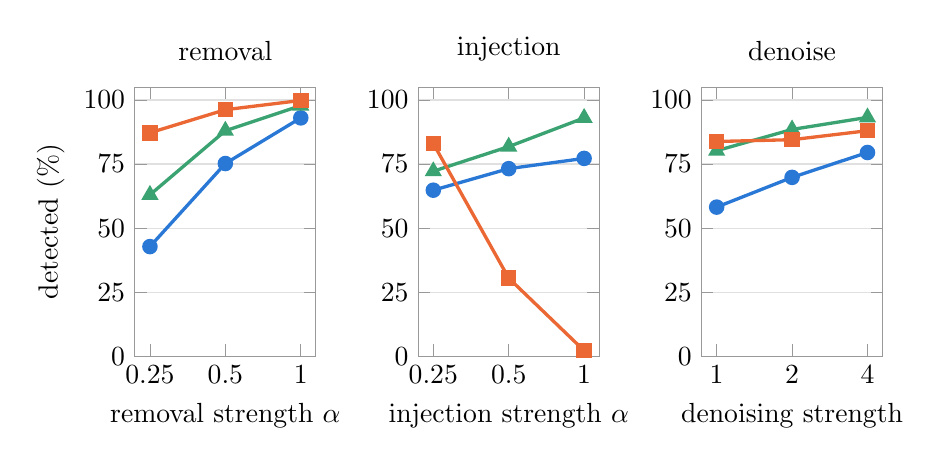
\begin{tikzpicture}\begin{groupplot}[group style={group size=3 by 1, horizontal sep=1.3cm},width=0.32\linewidth, height=5cm, ymin=0, ymax=105, ytick={0,25,50,75,100}]
\nextgroupplot[title={removal}, xlabel={removal strength $\alpha$}, xmode=log, log basis x=2, xtick={0.25,0.5,1}, xticklabels={0.25,0.5,1}, ylabel={detected (\%)}, legend to name=strengthlegend, legend columns=3]
\addplot[color=seriesA, mark=*, mark size=2.2pt, line width=1.2pt] coordinates {(0.25,42.8) (0.5,75.2) (1,93.0)};
\addplot[color=seriesC, mark=triangle*, mark size=2.4pt, line width=1.2pt] coordinates {(0.25,63.0) (0.5,88.0) (1,97.8)};
\addplot[color=seriesB, mark=square*, mark size=2.2pt, line width=1.2pt] coordinates {(0.25,87.2) (0.5,96.2) (1,99.8)};
\legend{XGBoost, Stacking (LR), PCE rule}
\nextgroupplot[title={injection}, xlabel={injection strength $\alpha$}, xmode=log, log basis x=2, xtick={0.25,0.5,1}, xticklabels={0.25,0.5,1}]
\addplot[color=seriesA, mark=*, mark size=2.2pt, line width=1.2pt] coordinates {(0.25,64.8) (0.5,73.2) (1,77.2)};
\addplot[color=seriesC, mark=triangle*, mark size=2.4pt, line width=1.2pt] coordinates {(0.25,72.2) (0.5,81.8) (1,93.0)};
\addplot[color=seriesB, mark=square*, mark size=2.2pt, line width=1.2pt] coordinates {(0.25,83.0) (0.5,30.5) (1,2.2)};
\nextgroupplot[title={denoise}, xlabel={denoising strength}, xmode=log, log basis x=2, xtick={1,2,4}, xticklabels={1,2,4}]
\addplot[color=seriesA, mark=*, mark size=2.2pt, line width=1.2pt] coordinates {(1,58.2) (2,69.8) (4,79.5)};
\addplot[color=seriesC, mark=triangle*, mark size=2.4pt, line width=1.2pt] coordinates {(1,80.2) (2,88.5) (4,93.2)};
\addplot[color=seriesB, mark=square*, mark size=2.2pt, line width=1.2pt] coordinates {(1,83.8) (2,84.5) (4,88.0)};
\end{groupplot}\end{tikzpicture}\\[2pt]\ref{strengthlegend}\caption{Attack strength vs detection (VISION attacks, realistic, 5-fold). The PCE rule ``detects'' removal only because low PCE is its sign of non-genuine; it misses injection, where the victim's fingerprint is matched.}\label{fig:strength}\end{figure}
\section{PRNU injected into AI-generated video}
Khan et al.\ (2025) transfer a camera's PRNU into AI-generated \emph{images} so that they pass source verification. We apply the same attack to video: the attacker estimates the fingerprint of a real camera from that camera's own videos and adds it to every frame of an AI clip, which is then encoded like all our clips. Table~\ref{tab:khanai} gives the share of clips accepted as genuine (PCE rule: PCE$_0$ with the claimed camera above 60; models: predicted \emph{organic}). GenVidBench clips are from the 5-fold test folds; GenBuster generators were never seen in training.
\begin{table}[H]\centering\small\caption{AI clips accepted as genuine camera footage (\%, lower is better for the defender).}\label{tab:khanai}\begin{tabular}{lrrrrrr}\toprule & \multicolumn{3}{c}{GenVidBench (seen generators)} & \multicolumn{3}{c}{GenBuster (unseen generators)} \\\cmidrule(lr){2-4}\cmidrule(lr){5-7} Detector & plain & $\alpha$=0.5 & $\alpha$=1 & plain & $\alpha$=0.5 & $\alpha$=1 \\\midrule
Khan et al.~2025 \cite{khan2025}, AI images & \multicolumn{6}{c}{85.5 (images, average)} \\\midrule
PCE rule & 0 & 84 & 98 & 0 & 77 & 96 \\
SVM & 5 & 4 & 2 & 6 & 6 & 3 \\
XGBoost & 5 & 2 & 0 & 6 & 3 & 1 \\
GRU & 3 & 2 & 0 & 5 & 3 & 0 \\
1D-CNN & 5 & 2 & 0 & 10 & 4 & 0 \\
Transformer & 6 & 3 & 1 & 6 & 4 & 1 \\
ViT (residual) & 1 & 1 & 0 & 15 & 9 & 4 \\
Ens.\ all & 3 & 2 & 0 & 4 & 3 & 0 \\
Stacking (LR) & 1 & 0 & 0 & 1 & 2 & 1 \\
\bottomrule\end{tabular}\end{table}
Injecting a camera's PRNU does not hide the AI origin: of the injected GenVidBench clips, Stacking (LR) calls 99\% synthetic, 1\% manipulated and 0\% organic. The injection makes the clip match the camera for the PCE rule, but it does not remove the other traces the models use (Noiseprint statistics, residual and temporal patterns).
\section{Cross-dataset test}
FloreView cameras are split by their PRNU baseline: 10 of 45 cameras have a usable video PRNU (attribution $\geq$ 50\%); the others are modern phones whose stabilisation removes it.
\begin{table}[H]\centering\small\caption{Cross-dataset detection rate (\%), models trained on VISION + ACID + GenVidBench (fixed split).}\label{tab:cross}\begin{tabular}{p{6.4cm}rrrrrrr}\toprule Condition & $n$ & PCE & XGB & GRU & ViT & Ens. & Stack \\\midrule
FloreView genuine, stabilised (no PRNU) & 1361 & 0 & 49 & 33 & 88 & 45 & 73 \\
FloreView genuine, usable PRNU & 355 & 62 & 78 & 57 & 96 & 76 & 91 \\
GenBuster AI & 600 & 100 & 73 & 62 & 84 & 76 & 97 \\
GenBuster AI + WA-like & 600 & 100 & 34 & 32 & 37 & 40 & 42 \\
GenBuster AI + YT-like & 600 & 100 & 75 & 53 & 78 & 70 & 91 \\
GenBuster AI + injected PRNU, $\alpha$=0.5 & 600 & 23 & 79 & 79 & 90 & 84 & 97 \\
GenBuster AI + injected PRNU, $\alpha$=1 & 600 & 4 & 86 & 86 & 95 & 88 & 97 \\
\bottomrule\end{tabular}\end{table}
\section{Feature ablation (RQ1)}
\begin{figure}[H]\centering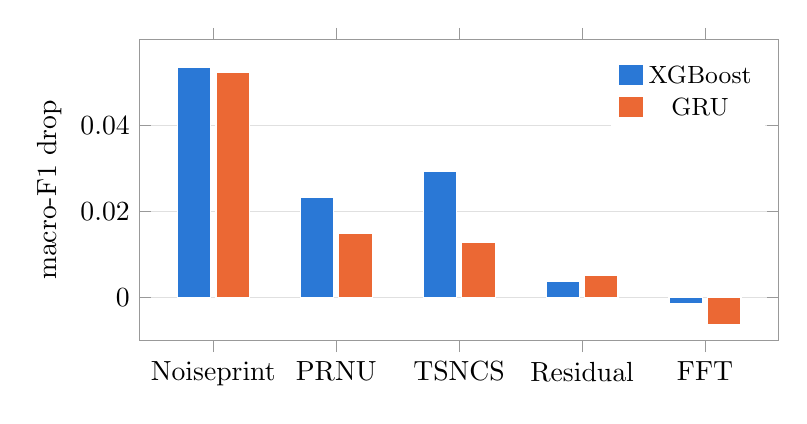
\begin{tikzpicture}\begin{axis}[ybar, bar width=12pt, width=0.8\linewidth, height=5.4cm,symbolic x coords={Noiseprint,PRNU,TSNCS,Residual,FFT}, xtick=data, ymin=-0.01, ylabel={macro-F1 drop}, enlarge x limits=0.15,scaled y ticks=false, yticklabel style={/pgf/number format/fixed, /pgf/number format/precision=2},legend style={at={(0.98,0.95)}, anchor=north east}, legend image code/.code={\draw[#1, draw=none] (0cm,-0.1cm) rectangle (0.3cm,0.15cm);}]
\addplot[fill=seriesA, draw=white] coordinates {(Noiseprint,0.0536) (PRNU,0.0233) (TSNCS,0.0293) (Residual,0.0038) (FFT,-0.0014)};
\addplot[fill=seriesB, draw=white] coordinates {(Noiseprint,0.0524) (PRNU,0.0148) (TSNCS,0.0129) (Residual,0.0051) (FFT,-0.0062)};
\legend{XGBoost, GRU}\end{axis}\end{tikzpicture}\caption{Drop in macro F1 when one feature group is removed (realistic, 5-fold, 5 frames). Larger = more important.}\label{fig:ablation}\end{figure}
\begin{table}[H]\centering\small\caption{Macro-F1 drop per feature group and model (5-fold, 5 frames).}\begin{tabular}{llccccc}\toprule Setup & Removed group & SVM & XGB & GRU & CNN & Transf. \\\midrule
realistic & Noiseprint & 0.053 & 0.054 & 0.052 & 0.048 & 0.067 \\
realistic & PRNU & 0.006 & 0.023 & 0.015 & 0.005 & 0.014 \\
realistic & TSNCS & 0.016 & 0.029 & 0.013 & 0.015 & 0.013 \\
realistic & Residual & 0.001 & 0.004 & 0.005 & -0.001 & 0.004 \\
realistic & FFT & 0.001 & -0.001 & -0.006 & 0.003 & 0.005 \\
controlled & Noiseprint & 0.054 & 0.046 & 0.047 & 0.062 & 0.054 \\
controlled & PRNU & 0.014 & 0.025 & 0.006 & 0.019 & 0.011 \\
controlled & TSNCS & 0.013 & 0.027 & 0.011 & 0.019 & 0.011 \\
controlled & Residual & 0.000 & 0.001 & 0.003 & 0.006 & 0.014 \\
controlled & FFT & -0.001 & 0.003 & -0.003 & 0.003 & 0.004 \\
\bottomrule\end{tabular}\end{table}
\section{Comparison with the base papers}
The base papers solve related but different tasks, so each is compared on its own terms. Literature values are taken from the papers as reported; protocols differ (noted per table).
\subsection{Camera identification: PDC-ViT (Elharrouss et al.~2025)}
PDC-ViT is a learned camera-identification model (80/20 train-test split, every camera seen in training). The closest component of HVPF is the training-free PRNU baseline (Step 4): fingerprints from flat videos, tested on natural videos, closed-set over all cameras of the dataset; verification at PCE$_0>60$. Our ViT shares PDC-ViT's input size but answers a different question (provenance class, not camera identity), on camera models it never saw in training.
\begin{table}[H]\centering\small\caption{Camera identification. Accuracy = closed-set attribution; FNR/FPR = verification.}\setlength{\tabcolsep}{4pt}\begin{tabular}{llrrrr}\toprule Method & Dataset (cameras) & Accuracy (\%) & FNR (\%) & FPR (\%) & EER (\%) \\\midrule
PDC-ViT \cite{pdcvit} & VISION (35) & 94.30 & -- & -- & -- \\
HVPF PRNU & VISION (35) & 73.4 & 36.2 & 0.00 & 18.3 \\
HVPF PRNU & VISION (21 non-stabilised) & 100.0 & -- & -- & -- \\
\midrule PRNU \cite{pdcvit} & Video-ACID + WA (26) & -- & 41.9 & 3.6 & -- \\
WA-PRNU \cite{pdcvit} & Video-ACID + WA (26) & -- & 28.06 & 2.8 & -- \\
PDC-ViT \cite{pdcvit} & Video-ACID + WA (26) & 74.77 & 23.4 & 0.92 & -- \\
HVPF PRNU & Video-ACID (44) & 59.1 & 59.6 & 0.00 & 25.5 \\
\midrule HVPF PRNU & FloreView (45) & 26.2 & 80.8 & 0.00 & 38.8 \\
\bottomrule\end{tabular}\end{table}
PRNU matching needs no training and is perfect on non-stabilised VISION cameras, above PDC-ViT; electronic stabilisation is what lowers the all-camera figures. Our verification threshold is strict (FPR 0\%), so FNR is higher than PDC-ViT's (FPR 0.92\%); the EER gives a threshold-free view. PDC-ViT was not tested on manipulated or synthetic video, and no base paper uses FloreView.
\subsection{PRNU-transfer attack: Khan et al.~2025}
Khan et al.\ report that 85.5\% of PRNU-transferred images pass source verification. Table~\ref{tab:khanai} covers their AI-image case on video; Table~\ref{tab:khancam} covers transfer between real cameras (our \emph{injection} attack). Compromise rate = share of injected clips accepted as genuine (realistic, 5-fold, 5 frames).
\begin{table}[H]\centering\small\caption{Compromise rate of PRNU injection between cameras (\%, lower is better for the defender).}\label{tab:khancam}\begin{tabular}{lrrrrrr}\toprule & \multicolumn{3}{c}{Injection strength $\alpha$} & \multicolumn{2}{c}{$\alpha$=0.5, re-shared} & \\\cmidrule(lr){2-4}\cmidrule(lr){5-6} Detector & 0.25 & 0.5 & 1 & WA-like & YT-like & All \\\midrule
Khan et al.~2025 \cite{khan2025}, images & \multicolumn{5}{c}{--} & 85.5 \\\midrule
PCE rule & 17 & 70 & 98 & 2 & 26 & 42 \\
SVM & 28 & 23 & 8 & 24 & 27 & 22 \\
XGBoost & 32 & 18 & 2 & 24 & 30 & 22 \\
GRU & 32 & 21 & 4 & 18 & 26 & 20 \\
1D-CNN & 30 & 22 & 6 & 22 & 24 & 21 \\
Transformer & 32 & 20 & 5 & 14 & 26 & 19 \\
ViT (residual) & 36 & 26 & 11 & 21 & 44 & 27 \\
Ens.\ all & 28 & 18 & 2 & 18 & 26 & 19 \\
Stacking (LR) & 26 & 14 & 1 & 13 & 26 & 16 \\
\bottomrule\end{tabular}\end{table}
A full-strength injection fools the PCE rule in 98\% of the clips, in line with Khan et al.; the best learned detector lets through only 1.2\%. Weak injections ($\alpha$=0.25) rarely fool PCE but are also harder for the models to spot.
\subsection{Low false-positive operation: Bao et al.~2024}
Bao et al.\ detect frame deletion (a different manipulation) from inter-frame noise consistency, the idea behind TSNCS, and stress performance at low false-positive rates; their results are given as ROC curves only. Table~\ref{tab:lowfpr} reports HVPF at the same kind of operating points: share of non-genuine clips detected while at most 1, 5 or 10\% of genuine clips are flagged.
\begin{table}[H]\centering\small\caption{Detection rate of non-genuine clips at fixed false-positive rates (realistic, 5-fold, 5 frames).}\label{tab:lowfpr}\begin{tabular}{lrrr}\toprule Detector & FPR 1\% & FPR 5\% & FPR 10\% \\\midrule
PCE rule & 5.3 & 9.9 & 16.3 \\
SVM & 34.4 & 55.5 & 65.7 \\
XGBoost & 48.2 & 62.3 & 72.0 \\
GRU & 42.7 & 60.9 & 69.9 \\
1D-CNN & 28.5 & 55.9 & 67.0 \\
Transformer & 44.5 & 60.4 & 69.8 \\
ViT (residual) & 48.6 & 61.3 & 71.6 \\
Ens.\ all & 52.0 & 66.2 & 75.2 \\
Stacking (LR) & 56.4 & 70.5 & 78.7 \\
\bottomrule\end{tabular}\end{table}
\subsection{What the base papers do not cover}\begin{itemize}
\item PRNU injection and removal attacks on \emph{video}, including platform-like re-sharing (Khan et al.\ test images only).
\item PRNU transfer into AI-generated \emph{video}, tested against unseen generators.
\item Camera identification under attack (PDC-ViT reports clean data only).
\item FloreView as an unseen-camera test set.
\item One model that separates genuine, manipulated and AI-generated video.
\end{itemize}
\section{Limitations and next steps}\begin{itemize}
\item Phones whose electronic stabilisation removes the PRNU (most FloreView cameras): the feature-based models still
      miss about half of them; the ViT recognises most. More such phones in training would help every model.
\item Platform-like copies make attacks and unseen-generator AI clips much harder to see, WhatsApp-like re-encoding most
      of all (Tables~\ref{tab:cond} and \ref{tab:cross}). All platform copies of fakes are simulated; only genuine VISION
      videos have real WhatsApp/YouTube copies.
\item The manipulated class comes from 400 videos of the 35 VISION cameras, and all attacks are our own implementation;
      ACID cameras appear only as genuine re-encodes.
\item The ViT sees one I-frame at a time and was run at 5 frames; 10-frame and multi-frame versions are the natural next step.
\item Sora is represented by only 51 clips; more high-quality modern generators are needed.
\end{itemize}
\begin{thebibliography}{9}
\bibitem{pdcvit} O.~Elharrouss et al., ``PDC-ViT: source camera identification using pixel difference convolution and
  vision transformer,'' \emph{Neural Computing and Applications}, 2025, doi:10.1007/s00521-025-11004-z.
\bibitem{khan2025} Khan, Hasan, Islam, ``Spoofing camera source attribution via PRNU transfer attacks,''
  \emph{ISC 2025}, Springer LNCS 16186, pp.~279--299, 2025.
\bibitem{bao2024} Bao et al., ``Anti-forensics video forgery detection via noise transfer matrix,''
  \emph{Sensors} 24(16):5341, 2024, doi:10.3390/s24165341.
\end{thebibliography}
\end{document}
